\documentclass[a4paper, 12pt]{article}

% https://tex.stackexchange.com/a/596136

\usepackage[utf8]{inputenc}
\usepackage{tikz}
\usetikzlibrary{arrows.meta}
\tikzset{% common styles of tikz pictures elements
  treenode/.style = {shape=rectangle, rounded corners,
                     draw, align=center, 
                     minimum height=2ex, text depth=0.25ex,
                     top color=white, bottom color=blue!20},
  root/.style     = {treenode, font=\Large\rmfamily, bottom color=red!30},
  env/.style      = {treenode, font=\ttfamily\normalsize},
}

\begin{document}

\begin{figure}
    \centering
    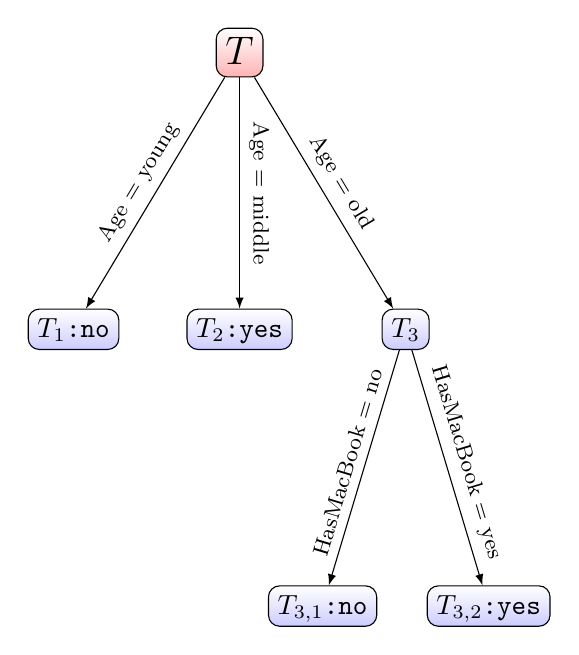
\begin{tikzpicture}[% local settings for tree
            %grow                     = right,
            sibling distance         = 6em,
            level distance           = 10em,
            edge from parent/.style  = {draw, -latex},
            every node/.append style = {font=\footnotesize},
            sloped
        ]
        \node [root] {$T$}    % root node, here tree start, after it are children
        child { node [env] {$T_1$:no}
                edge from parent node [above] {Age = young}}
        child { node [env] {$T_2$:yes}
                edge from parent node [above] {Age = middle}}
        child { node [env] {$T_3$}
                child { node [env] {$T_{3, 1}$:no}
                        edge from parent node [above] {HasMacBook = no}}
                child { node [env] {$T_{3, 2}$:yes}
                        edge from parent node [above] {HasMacBook = yes}}
                edge from parent node [above] {Age = old}}
        ;
    \end{tikzpicture}
    \caption{Decision tree}
    \label{fig:decision-tree}
\end{figure}

\end{document}
